\makesection{Recommender Systems}

\begin{frame}{RecSys}
    \begin{wrapfigure}{r}{0.45\textwidth}
    \centering
    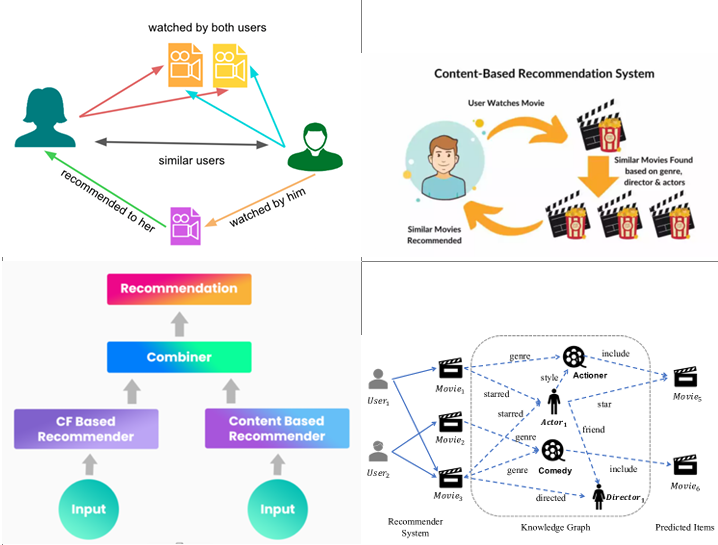
\includegraphics[width=0.45\textwidth]{images/RecSys.png}
    \caption{Tipologie di RecSys}
\end{wrapfigure}

Un sistema di raccomandazione è un software che suggerisce all'utente elementi di interesse (prodotti, servizi, contenuti) basandosi sulle preferenze e i comportamenti passati. Ampiamente usati in e-commerce, social network, servizi di streaming e piattaforme di informazione, questi sistemi migliorano l'esperienza utente, aumentano la soddisfazione e la fidelizzazione, e aiutano a scoprire nuovi contenuti. Utilizzano algoritmi di apprendimento automatico e intelligenza artificiale per analizzare i dati e generare raccomandazioni personalizzate.
\end{frame}

\begin{frame}{Valutazione e problemi dei RecSys}
    \begin{block}{Valutazione}   
Per valutare un RecSys si possono usare diverse metriche come il MAE (Mean Absolute Error) che misura la differenza tra il valore predetto e il valore reale, l'NDGC che misura la qualità delle raccomandazioni, la diversity che misura la varietà delle raccomandazioni, la coverage che misura la percentuale di elementi raccomandati, la recall che misura la capacità di un modello di raccomandare gli item rilevanti per un utente
\end{block}
\begin{alertblock}{Problemi}

I RecSys possono presentare problemi di Cold Start, quando non si hanno informazioni sufficienti per fare raccomandazioni, di More of the Same, quando si raccomandano sempre gli stessi elementi, la vulnerabilità agli attacchi (come recensioni false).
\end{alertblock}
\end{frame}